\documentclass[output=paper]{langscibook} 
\author{Eleanor Glewwe\affiliation{University of California, Los Angeles}}
\title{Efik Nominal Tonal Alternations as Phrasal Morphology}

% \chapterDOI{} %will be filled in at production
 
\abstract{Certain Efik nominal constructions exhibit fixed tonal melodies that overwrite nouns’ underlying tones. Previous analyses of these alternations (\citealt{Welmers1973}, \citealt{Kim1974}, \citealt{Cook1985}) are purely phonological. Working in a constraint-based framework, I propose that the tonal alternations are actually phrasal morphology \citep{McPherson2014}. The tonal melodies are overlays encoded in lexicalized constructional schemas that relate idiosyncratic phrasal phonology with specific syntactic constructions. The constructional schemas are enforced by constraints. The Efik case extends the observed range of phrasal morphology by demonstrating that constructional schema constraints and phonological constraints can interact to determine a construction’s surface tones.}
\maketitle

\begin{document}

\section{Efik Nominal Tonal Alternations}

Efik (Niger-Congo: Benue-Congo: Cross River) is a language spoken in Cross River State in southeastern Nigeria \citep{Cook1985}. It has two tones, high (H) and low (L), which may combine in a single syllable to produce falling (HL) and rising (LH) tones \citep{Welmers1968}. Additionally, there is a downstepped high tone (\textsuperscript{$\downarrow$}H) whose pitch is lower than H but higher than L. I analyze \textsuperscript{$\downarrow$}H as an H after a floating L. 

In certain nominal constructions, including noun-noun compounds, adjective-noun constructions, and genitive constructions, nouns exhibit tonal alternations. For instance, in the noun-noun compound ‘dog house,’ the underlyingly H-H noun \textit{ébwá} ‘dog’ is realized as H-L after the underlyingly H-L noun \textit{úfɔk} ‘house’: 

\ea \label{ex:glewwe:1}
\gll /úfɔk  ébwá/ {${\rightarrow}$  [úfɔk ébwà]}\\ 
     house dog {}\\
\glt ‘dog house’
\z

The complete patterns of nominal tonal alternations in compounds are given in \tabref{tab:glewwe:1}. These patterns were reported by \citealt{Welmers1968} and \citealt{Cook1985} and confirmed with new data elicited from six native speakers of Efik. 

\begin{table}
    \begin{tabular}{llccccccc}
        \lsptoprule
        \multicolumn{2}{p{3cm}}{\multirow{4}{3cm}{Underlying tonal shape of first noun}} &  \multicolumn{7}{c}{Underlying Tonal Shape of Second Noun}\\
        \cmidrule(lr){3-9}
        & & \multicolumn{4}{c}{Group 1} & \multicolumn{3}{c}{Group 2}\\\cmidrule(lr){3-6}\cmidrule(lr){7-9}
        & & H-H & H-HL & H-L & L-L & L-H & L-HL\footnotemark{} & H-\textsuperscript{$\downarrow$}H\\
        \midrule
         Alternation 1 & H-H & & & & & & &  \\
         & H-L & & & & & & &  \\
         & L-L & \multicolumn{4}{c}{H-L} & \multicolumn{3}{c}{H-\textsuperscript{$\downarrow$}H} \\
         & L-H  & & & & & & & \\
         & H-H & & & & & & & \\
         \midrule
        Alternation 2 & H-HL  & \multicolumn{4}{c}{L-L}&\multicolumn{3}{c}{L-H}\\
         & L-HL  & & & & & & & \\
        \lspbottomrule
    \end{tabular}
    \caption{Surface Tones on the Second Noun in Noun-Noun Compounds}
    \label{tab:glewwe:1}
\end{table}

\footnotetext{ L-HL nouns actually preserve their final fall, surfacing as H-\textsuperscript{$\downarrow$}HL and L-HL under Alternations 1 and 2, respectively.} 


As \tabref{tab:glewwe:1} shows, disyllabic nouns occur in seven tonal shapes: H-H, H-L, L-H, L-L, H-HL, L-HL, and H-\textsuperscript{$\downarrow$}H \citep[86]{Welmers1968}. Nouns longer than two syllables still exhibit one of these seven tonal melodies. In a noun-noun compound, only the tones of the second (non-head) noun alternate; the tones of the first noun surface unchanged. The seven nominal tonal shapes can be divided into two groups according to the pattern of alternations they exhibit. Group 1 comprises H-H, H-HL, H-L, and L-L nouns while Group 2 comprises L-H, L-HL, and H-\textsuperscript{$\downarrow$}H nouns (the terms Group 1 and Group 2 come from \citealt{Welmers1968}). Additionally, there are two alternation patterns in compounds, triggered by two different sets of nouns. Alternation 1 is triggered by first nouns with tonal shapes ending in H or L while Alternation 2 is triggered by first nouns with tonal shapes end in HL (Alternation 1 and Alternation 2 are also Welmers’ terms). Each tonal shape group exhibits a different output under each of the two tonal alternations, yielding a total of four patterns. After a noun ending in H or L, Group 1 nouns surface as H-L, and after a noun ending in HL, they surface as L-L. Group 2 nouns surface as H-\textsuperscript{$\downarrow$}H after a noun ending in H or L and as L-H after a noun ending in HL. Thus in \REF{ex:glewwe:1}, the noun \textit{ébwá} ‘dog’ surfaces as H-L in the compound ‘dog house’ because it is a Group 1 noun (with underlying tones H-H) and it occurs after the noun \textit{úfɔk} ‘house,’ which ends in L.  

While complex, these tonal alternation patterns can be summarized in a few generalizations. There are essentially two tonal melodies, HL, which corresponds to Alternation 1, and L, which corresponds to Alternation 2. The melody HL occurs after nouns ending in a level tone (H or L) while the melody L occurs after nouns ending in a falling tone (HL). The surface melodies H-\textsuperscript{$\downarrow$}H and L-H exhibit the melodies HL and L, respectively, but instead of continuing to the end of the word, the melodies stop before an H that is the final tone of the word. H-\textsuperscript{$\downarrow$}H and L-H arise in Group 2 nouns, which differ from Group 1 nouns in that their tonal shapes contain an H after an L (in H-\textsuperscript{$\downarrow$}H nouns, the L that the second H follows is unassociated, manifesting as downstep). Thus in Group 2 nouns the tonal melodies HL and L extend only as far as the H that followed the original underlying L and no further, leaving that H to be realized on the second syllable of the noun. 

In \REF{ex:glewwe:2}, I provide a few more compounds that illustrate the tonal alternation patterns in \tabref{tab:glewwe:1}: 

\ea\label{ex:glewwe:2} 
\ea \label{ex:glewwe:2a}
\gll /ùbóm íják/  ${\rightarrow}$ [ùbóm íjàk]  Alt. 1 Group 1 H-L\\ 
       boat fish\\
\glt ‘fish boat’ 

\ex\label{ex:glewwe:2b}
\gll   /ɔfɔŋ ùsàn/  ${\rightarrow}$ [ɔfɔŋ úsàn]  Alt. 1 Group 1 H-L\\
       cloth dish\\
\glt ‘dish cloth’ 

\ex\label{ex:glewwe:2c}
\gll   /ùsàn èjɨm/  ${\rightarrow}$ [ùsàn é\textsuperscript{$\downarrow$}jɨm]  Alt. 1 Group 2 H-\textsuperscript{$\downarrow$}H\\
       dish onion\\
\glt   ‘onion dish’ 

\ex\label{ex:glewwe:2d}
\gll   /úfɔk ì\~{w}áŋ/  ${\rightarrow}$ [úfɔk í\textsuperscript{$\downarrow$}\~{w}áŋ]  Alt. 1 Group 2 H-\textsuperscript{$\downarrow$}H\\
       house farm\\
\glt   ‘farm house’

\ex\label{ex:glewwe:2e}
\gll   /íkwâ ébwá/ ${\rightarrow}$ [íkwâ èbwà]  Alt. 2 Group 1 L-L\\
       knife dog\\
\glt   ‘dog knife’

\ex\label{ex:glewwe:2f}
\gll   /à\~{w}â úkwàk/ ${\rightarrow}$ [à\~{w}â ùkwàk]  Alt. 2 Group 1 L-L\\
       cat iron\\
\glt   ‘iron cat’

\ex\label{ex:glewwe:2g}
\gll   /íkwâ í\textsuperscript{$\downarrow$}nwɛn/ ${\rightarrow}$ [íkwâ ìnwɛn]  Alt. 2 Group 2 L-H\\
       knife bird\\
\glt   ‘bird knife’

\ex\label{ex:glewwe:2h}
\gll   /à\~{w}â í\textsuperscript{$\downarrow$}nwɛn/ ${\rightarrow}$ [à\~{w}â ìnwɛn]  Alt. 2 Group 2 L-H\\
       cat bird\\
\glt   ‘bird cat’
\z
\z

Previous analyses of the Efik nominal tonal alternations (\citealt{Welmers1973}, \citealt{Kim1974}, \citealt{Cook1985}) are purely phonological. Only \citealt{Cook1985} is fully elaborated. For noun-noun compounds, Cook posits a construction marker /H L/, that is, a high tone followed by a low tone with no segmental material, that occurs between the two nouns of the compound (e.g. /ú-fɔk  \'{}   \`{}  é-bwá/ ‘dog house’). He derives the surface tones of the second noun with three phonological rules. Two are tonal assimilation rules triggered by floating tones. Assimilation to Floating L changes each H of a continuous string of Hs to L after a floating L (e.g. /  \`{}  ${\sigma}$\'{}  ${\sigma}$\'{}  ${\sigma}$\'{} / ${\rightarrow}$ [  \`{}  ${\sigma}$\`{}  ${\sigma}$\`{}  ${\sigma}$\`{}  ]) while Assimilation to Floating H changes a single L to H after a floating H and applies iteratively (e.g. /  \'{}   \`{}  ${\sigma}$\`{}  ${\sigma}$\`{}  ${\sigma}$\`{} / ${\rightarrow}$ [  \'{}   \'{}  ${\sigma}$\`{}  ${\sigma}$\`{}  ${\sigma}$\`{}  ] ${\rightarrow}$ [  \'{}   \'{}  ${\sigma}$\'{}  ${\sigma}$\`{}  ${\sigma}$\`{}  ]) \citep[193]{Cook1985}. These rules seem somewhat arbitrary. Why does a floating L affect a whole string of following Hs (Assimilation to Floating L) while a floating H affects only a single following L but can apply iteratively (Assimilation to Floating H)? Why do floating tones but not associated tones trigger these assimilations? 

These two assimilation rules have at least some application outside nominal constructions in Cook’s phonology of Efik, but the third rule that derives the tonal alternations in compounds is purely ad hoc. This rule, called L Copying, copies an initial L of a noun when that initial L is preceded by a word boundary and a floating tone. (Specifically, the L copies onto an open transition, a unit specific to Cook’s phonological analysis of Efik. An open transition is a segmental phoneme that is not audible but can bear a tone and occurs immediately after the initial vowel of most nouns.) L Copying’s sole role in the grammar is to ensure that tonal alternations in compounds and other nominal constructions come out right. In particular, it is needed to derive downstep where it is observed to occur. 

While Cook’s analysis can account for all four tonal alternation patterns in \figref{tab:glewwe:1}, the rules it relies on are unsatisfying. Moreover, it does not capture the generalizations stated above, namely that there are essentially two surface melodies, HL and L, and that consistent tonal properties of the first and second nouns in compounds give rise to the full set of four patterns. 

Instead of treating the nominal tonal alternations as purely phonological, I propose a phrasal morphology account for them. This analysis is presented in the following section. I then consider an alternative, constraint-based phonological account and argue that the phrasal morphology account is preferable. 

\section{A Phrasal Morphology Account} 

The phrasal morphology account I advocate treats the surface tones in Efik compounds as tonal melodies that are imposed in particular constructions. This approach is reminiscent of Harry \& \citegen{Hyman2014} approach to Kalabari nouns, which exhibit tonal alternations in many of the same constructions as in Efik. While they do not provide a fully implemented analysis, Harry \& Hyman argue for a constructional, rather than a purely phonological, approach in which Kalabari nouns in certain constructions, including compounds and genitive constructions, lose their underlying tones and are assigned a particular tonal melody. 

My analysis of Efik is couched in a different constructional framework, that of \citealt{McPherson2014}. In McPherson’s framework, lexicalized constructional schemas relate idiosyncratic phrasal phonology with particular syntactic constructions. For example, in specific syntactic constructions, certain word classes may impose tonal overlays on other words. In the case of Efik noun-noun compounds, it will be the first (head) noun that imposes a tonal overlay on the second (non-head) noun. Recall the generalizations from §1: the second nouns in compounds exhibit two melodies, HL and L, with HL occurring after a first noun ending in a level tone and L occurring after a first noun ending in a falling tone. In keeping with McPherson’s framework, there is a constructional schema for Efik noun-noun compounds that specifies a tonal overlay with two allomorphs, \{HL\} and \{L\}, and the environment in which each allomorph occurs. The constructional schema is associated with a constraint that enforces the application of the appropriate tonal overlay, and the interaction of this constructional schema constraint with other phonological constraints gives rise to the full range of surface tones seen on the second nouns of compounds. 

The constructional schema for Efik compounds is given in \figref{fig:glewwe:2}.

  
\begin{figure}
% % 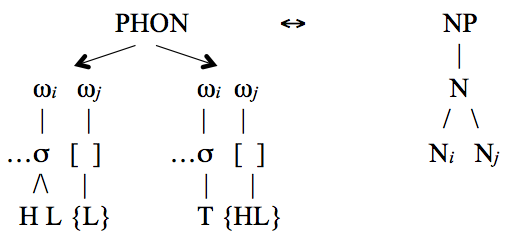
\includegraphics[width=\textwidth]{figures/glewwe-img1.png}
\begin{forest} baseline
[PHON, s sep=1cm
    [,l=0mm,l sep=0mm,shape=coordinate,edge=->%dummy node
        [ω\textsubscript{i},no edge,l=0mm,l sep=0mm [...σ [H] [L]]]
        [ω\textsubscript{j},no edge,l=0mm,l sep=0mm [{[~]} [\{L\}]]]
    ]
    [,l=0mm,l sep=0mm,shape=coordinate,edge=->%dummy node
        [ω\textsubscript{i},no edge,l=0mm,l sep=0mm [...σ [T]]]
        [ω\textsubscript{j},no edge,l=0mm,l sep=0mm [{[~]} [\{HL\}]]]
    ]
]
\end{forest}↔\begin{forest} baseline
[NP [N [N\textsubscript{i}] [N\textsubscript{j}] ] ]
\end{forest}
\caption{Constructional schema for Efik noun-noun compounds}
\label{fig:glewwe:2}
\end{figure}

Constructional schemas show the correspondence of idiosyncratic phonology, including tonal overlays, with specific syntactic structures. The schema in \figref{fig:glewwe:2} states that in a noun-noun compound, if the first noun ends in a falling tone HL, the tonal overlay \{L\} is imposed on the second noun, and if the first noun ends in a syllable with a single tone (H or L) associated to it, the tonal overlay \{HL\} is imposed on the second noun. 

This schema is enforced with the single constructional schema constraint N~N\textsuperscript{(H)L}, which is satisfied when the correct allomorph of the tonal overlay is imposed on the second noun of a compound. N~N\textsuperscript{(H)L} counts one violation for each associated tone in the output that does not match the overlay (we will see later why its evaluation is not binary). Following \citet{McPherson2014}, the complementary faithfulness constraint I use is \textsc{Faith(T).} One violation of \textsc{Faith(T)} is incurred when a word’s tones in the output do not match its tones in the input. 

The tableau in \figref{fig:glewwe:3} shows the derivation of the surface tone pattern H-L (Group 1 Alternation 1) with the compound \textit{úfɔk} \textit{ébwà} ‘dog house.’ A superscript on a word indicates that a tonal overlay has been imposed, whether partially or fully.  

  
\begin{figure}
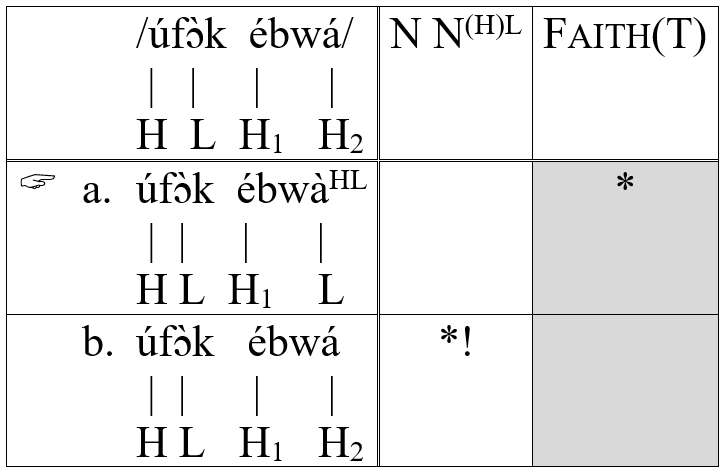
\includegraphics[width=\textwidth]{figures/glewwe-img2.png}
\caption{Tableau for \textup{úfɔk ébwà}}
\label{fig:glewwe:3}
\end{figure}

The first noun in the compound, /úfɔk/, ends in L, so according to the constructional schema in \figref{fig:glewwe:2} it seeks to impose the overlay \{HL\} on the second noun, /ébwá/. The constructional schema constraint N~N\textsuperscript{(H)L} is violated if the tonal overlay is not exhaustively imposed. Candidate (b), the faithful candidate, only partially satisfies the overlay, realizing it on the first syllable of \textit{ebwa} but not imposing it over the final H of this word. The H on the final syllable of \textit{ebwa} does not match the tonal overlay, so one violation of N~N\textsuperscript{(H)L} is incurred. Candidate (a) imposes the overlay exhaustively and so does not violate the constructional schema constraint. It changes the tones of \textit{ebwa}, violating \textsc{Faith(T)}, but since N~N\textsuperscript{(H)L} >> \textsc{Faith(T)}, it is the winner. Note that I assume lexical tones can realize tonal overlays. Thus in the winner the first tone of the \{HL\} overlay is in fact the original first H of \textit{ébwá}; this lexical tone is maintained since it can realize the overlay. The same is true in candidate (b). 

The tableau in \figref{fig:glewwe:4} shows the derivation of the surface tones L-L (Group 1 Alternation 2) with the compound \textit{íkwâ} \textit{èbwà} ‘dog knife’: 

  
\begin{figure}
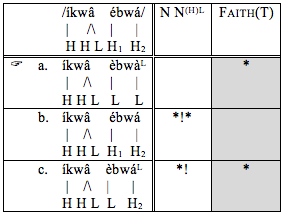
\includegraphics[width=\textwidth]{figures/glewwe-img3.png}
\caption{Tableau for \textup{íkwâ èbwà}}
\label{fig:glewwe:4}
\end{figure}

The first noun of the compound, /íkwâ/, ends in HL, so according to the constructional schema it seeks to impose the overlay \{L\} on /ébwá/. The faithful candidate, (b), does not impose the overlay at all, thereby incurring two violations of N~N\textsuperscript{(H)L}, and candidate (c) imposes the overlay only partially, incurring one violation of N~N\textsuperscript{(H)L}. Consequently, they both lose to candidate (a), which exhaustively imposes the overlay.     

Having accounted for the surface tones of Group 1 nouns in compounds, I now consider Group 2 nouns. The surface melodies that must be derived are H-\textsuperscript{$\downarrow$}H and L-H. As discussed in §1, Group 2 nouns (those with the tonal shapes L-H, L-HL, or H-\textsuperscript{$\downarrow$}H) differ from Group 1 nouns in that they contain an H after an L (the L is floating in H-\textsuperscript{$\downarrow$}H nouns). After nouns ending in a falling tone, Group 2 nouns have the surface tones L-H (Group 2 Alternation 2). These nouns do exhibit the melody of the \{L\} allomorph of the tonal overlay, but the noun’s original underlying H after the underlying L is preserved. That is, the imposition of the overlay is halted by the H after the L and does not extend beyond it. I therefore propose that an H following an L in the same word is preserved by the following special positional faithfulness constraint: 

\ea \label{ex:glewwe:3}
{\textsc{PreserveHPostL:} An associated H that follows an L (associated or not) within the same word in the input must be associated in the output.} \\
\z

This constraint, combined with the constructional schema constraint, derives the surface pattern L-H. The idea is that \textsc{PreserveHPostL} blocks the tonal overlay from proceeding past the H after the L. The tableau in \figref{fig:glewwe:5} illustrates this with the compound \textit{íkwâ} \textit{ìnwɛn} ‘bird knife’: 

  
\begin{figure}
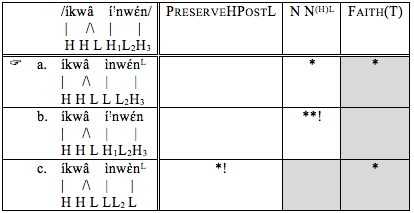
\includegraphics[width=\textwidth]{figures/glewwe-img4.png}
\caption{Tableau for \textup{íkwâ ìnwɛn}}
\label{fig:glewwe:5}
\end{figure}

Since the first noun of the compound, /íkwâ/, ends in HL, the constructional schema dictates that it impose the overlay \{L\} on /í\textsuperscript{$\downarrow$}nwɛn/. \textsc{PreserveHPostL} outranks N~N\textsuperscript{(H)L} and prevents exhaustive realization of the overlay, eliminating candidate (c). Because N~N\textsuperscript{(H)L} counts the number of tones that do not match the overlay, though, non-exhaustive realization, as in candidate (a), is still better than no realization, as in (b), so the winner is [íkwâ ìnwɛn\textsuperscript{L}]. 

The final surface melody to be derived is H-\textsuperscript{$\downarrow$}H (Group 2 Alternation 1). Group 2 nouns show the H-\textsuperscript{$\downarrow$}H pattern after nouns ending in H or L, so according to the constructional schema it is the \{HL\} overlay that is being imposed. The surface tones H-\textsuperscript{$\downarrow$}H do in fact show the \{HL\} overlay; the downstep is caused by the presence of an unassociated L. The question is why the L is unassociated. The final H in the H-\textsuperscript{$\downarrow$}H pattern can be explained by \textsc{PreserveHPostL}, which prevents the overlay from reaching the end of the word. If the \{HL\} overlay were fully realized on a Group 2 noun while the H after the L was preserved as well (i.e. if the \{HL\} overlay were realized on the first syllable of the noun and the H were preserved on the second syllable), the result would be an HLH sequence within a word. This sequence does not surface, so I claim that the constraint *HLH is active:

\ea\label{ex:glewwe:4} 
{*HLH: Within a word, don’t have the tonal sequence HLH, where all three tones are associated.\footnote{The domain of *HLH must ultimately be more specific because surface HLH sequences are permitted within a word in, for instance, inflected verb forms like \textit{á-sàŋá} ‘s/he is walking.’} }\\
\z

*HLH has been proposed for a variety of languages (\citealt{Cahill2007b}, \citealt{McPherson2016}) and seems to reflect a desire to avoid multiple sharp changes in pitch in close proximity (cf. \citegen{Hyman2007} Principle of Ups and Downs). There is independent evidence that *HLH is active within the word in Efik. As mentioned in §1, there are seven surface tonal shapes for Efik disyllabic nouns. All two-tone combinations of H and L are attested, as are the shapes H-HL, L-HL, and H-\textsuperscript{$\downarrow$}H, but the shapes H-LH and HL-H are not attested. Additionally, *HLH constrains the surface tones of reduplicated verb forms \citep{Glewwe2017}.

Because realizing the \{HL\} overlay and preserving a final H would violate *HLH, the L delinks, yielding the surface tones H-\textsuperscript{$\downarrow$}H. The tableau in \figref{fig:glewwe:6} shows the derivation of this pattern with the compound \textit{ùsàn} \textit{é\textsuperscript{$\downarrow$}}\textit{jɨm} ‘onion dish’: 

  
\begin{figure}
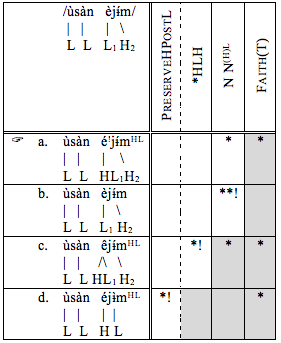
\includegraphics[width=\textwidth]{figures/glewwe-img5.png}
\caption{Tableau for \textup{ùsàn é}\textup{\textsuperscript{$\downarrow$}}\textup{jɨm}}
\label{fig:glewwe:6}
\end{figure}

As it ends in L, /ùsàn/ seeks to impose the overlay \{HL\} on /èjɨm/. Candidate (d) fully realizes the overlay, but it violates \textsc{PreserveHPostL}, so it is eliminated. Candidate (c) preserves the H following the L in /èjɨm/ and partially realizes the overlay by imposing the melody HL on the first syllable of \textit{ejɨm}, but the result violates *HLH. Candidates (a) and (b) respect \textsc{PreserveHPostL} and *HLH. The winning candidate, (a), delinks the L to avoid violating *HLH but still realizes the \{HL\} overlay better than the faithful candidate (b). The optimal form is thus the attested [ùsàn é\textsuperscript{$\downarrow$}jɨm]. 

The phrasal morphology account I have presented is able to handle the complete set of tonal alternations seen in Efik compounds. A potential alternative to this account is a purely phonological constraint-based analysis. In the next section, I consider what such an analysis might look like. 
 
\section{A Constraint-Based Phonological Account}

In working out a phonological account of the tonal alternations in Efik compounds, I adopt \citegen{Cook1985} construction marker /H L/, which occurs between the two nouns of a compound. The tones of the construction marker are compelled to surface by \textsc{RealizeMorpheme}. (\citealt{Gnanadesikan1997}, \citealt{Kurisu2001}, \citealt{Oostendorp2005}). The interaction of \textsc{RealizeMorpheme} with other phonological constraints gives rise to the four different surface patterns. 

The tableau in \figref{fig:glewwe:7} exemplifies the derivation of the surface tones H-L (Group 1 Alternation 1) with the compound \textit{úfɔk} \textit{ébwà} ‘dog house’: 

% \ea\label{ex:glewwe:}
\begin{figure}
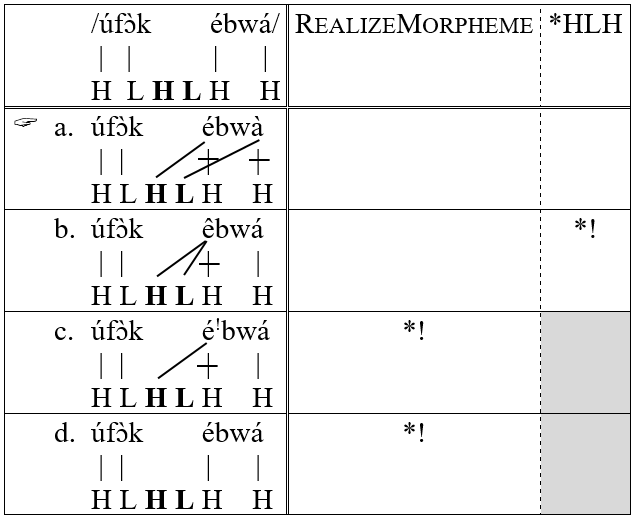
\includegraphics[width=\textwidth]{figures/glewwe-img6.png}
\caption{Tableau for \textup{úfɔk ébwà}}
\label{fig:glewwe:7}
\end{figure}


Candidates (c) and (d) do not realize both tones of the construction marker, so they are eliminated by \textsc{RealizeMorpheme}. *HLH, introduced above in the phrasal morphology account, rules out associating both tones of the construction marker to the first syllable of \textit{ebwa}, as in (b), so (a) is optimal. Note that \textsc{RealizeMorpheme} must be defined as being satisfied only if both tones of the construction marker are associated; otherwise, (c) would be as harmonic as (a). This is a departure from well-known formalizations of \textsc{RealizeMorpheme} that only require that \textit{some} element of the morpheme’s input be realized on the surface to satisfy the constraint (\citealt{Gnanadesikan1997}, \citealt{Oostendorp2005}). One might argue that in candidate (c) the L of the construction marker \textit{is} realized insofar as it has a surface phonological effect, namely, downstep. This would be in the spirit of approaches (e.g. \citealt{Gnanadesikan1997}) in which any detectable phonological effect of the morpheme counts as realization. However, for candidate (a) to be chosen over candidate (c), \textsc{RealizeMorpheme} must require both tones of the construction marker to be \textit{associated}, not merely audible in some way. I return to this subject below. 

Next I turn to the surface tones H-\textsuperscript{$\downarrow$}H (Group 2 Alternation 1). This is one of the patterns exhibited by Group 2 nouns, those with the tonal shapes L-H, L-HL, or H-\textsuperscript{$\downarrow$}H. The surface pattern H-\textsuperscript{$\downarrow$}H does show the HL melody of the construction marker, but the L is suppressed, appearing only as downstep, while the underlying H after the underlying L is preserved. To derive the behavior of Group 2 nouns, I make use of the constraint \textsc{PreserveHPostL} from the phrasal morphology account. 

The surface pattern H-\textsuperscript{$\downarrow$}H is exemplified by the compound \textit{ùsàn} \textit{é\textsuperscript{$\downarrow$}}\textit{jɨm} ‘onion dish.’ Notice that if the H on the second syllable of /èjɨm/ is preserved on the surface, as in [é\textsuperscript{$\downarrow$}jɨm], it means that the L of the construction marker /H L/ has not been associated. That is, only one tone of the construction marker is associated, meaning that this candidate violates \textsc{RealizeMorpheme} as defined above. In that case, one would expect the faithful candidate [ùsàn èjɨm], in which \textit{none} of the tones of the construction marker are associated, to win, since this candidate also violates \textsc{RealizeMorpheme} but is more faithful. Overcoming this problem requires a workaround. To ensure that the correct candidate wins, I allow \textsc{RealizeMorpheme} to count units of the morpheme being compelled to realize, so that its evaluation is no longer binary. In this case, the units of the morpheme are tones. Now the surface tones H-\textsuperscript{$\downarrow$}H can be derived, as shown in the tableau in \figref{fig:glewwe:8} for \textit{ùsàn} \textit{é\textsuperscript{$\downarrow$}}\textit{jɨm} ‘onion dish’: 

  
\begin{figure}
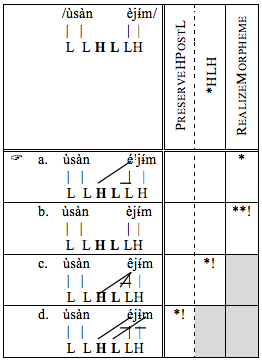
\includegraphics[width=\textwidth]{figures/glewwe-img7.png}
\caption{Tableau for \textup{ùsàn é}\textup{\textsuperscript{$\downarrow$}}\textup{jɨm}}
\label{fig:glewwe:8}
\end{figure}

Candidate (d) associates one tone of the construction marker to each syllable of \textit{ejɨm}, but this violates \textsc{PreserveHPostL}. Candidate (c) preserves the underlying H after the L by realizing the construction marker on the first syllable of \textit{ejɨm}, but this violates *HLH. The faithful candidate (b) incurs two violations of \textsc{RealizeMorpheme} while (a) only incurs one by partially realizing the construction marker, so (a) wins. 

If the downstep in candidate (a) could qualify as realization of the floating L of the construction marker and therefore exempt candidate (a) from violating \textsc{RealizeMorpheme,} candidate (b) would no longer need to incur two violations of the constraint to lose to candidate (a). The evaluation of \textsc{RealizeMorpheme} could then remain binary. We saw in the derivation of \textit{úfɔk} \textit{ébwà} (\figref{fig:glewwe:7}) that downstep cannot count as realization of the L of the construction marker, though, so this attempt to keep \textsc{RealizeMorpheme} binary will not work.   

I turn now to the surface tones L-L (Group 1 Alternation 2). This pattern arises in the compound \textit{íkwâ} \textit{èbwà} ‘dog knife.’ Group 1 nouns like \textit{ébwá} ‘dog’ surface as L-L instead of H-L when the preceding noun ends in a falling tone HL. For some reason, the H of the construction marker does not associate to the first syllable of the second noun when the first noun ends in HL. It seems, then, that the HL\#H (falling \# high) sequence is avoided, but this structure does not violate *HLH because it is not within a word. Some other markedness constraint must be devised to penalize this structure. I therefore put forth the following constraint: 

\ea \label{ex:glewwe:5}
{*HLH<3: Don’t have the tonal sequence HLH on fewer than three syllables.\footnote{This constraint must also be restricted to some domain, since HLH sequences on fewer than 3 syllables can arise elsewhere, e.g. on a subject prefix and following verb in \textit{ń-tjɛ-ɣɛ-tjɛ} \textsc{1sg-}sit\textsc{-neg{\textasciitilde}foc} ‘I’m not \textit{sitting}.’} }\\
\z

The constraint specifies that the HLH sequence must occur on fewer than three syllables to incur a violation because in a compound like \textit{úfɔk} \textit{ébwà} ‘dog house,’ there is an HLH sequence spanning three syllables, and the form is perfectly licit (see \citealt{McPherson2016} for another *HLH constraint with a configuration restriction). 

Realizing the H of the construction marker on the first syllable of the second noun when the first noun ends in the contour tone HL would violate *HLH<3, so the H of the construction marker changes to L. The tableau in \figref{fig:glewwe:9} shows how the surface tones L-L are derived for the compound \textit{íkwâ} \textit{èbwà} ‘dog knife’.

  
\begin{figure}
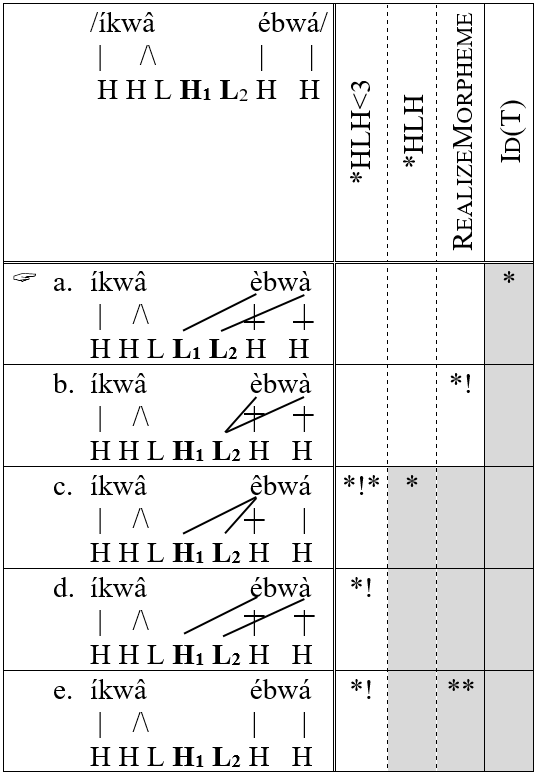
\includegraphics[width=\textwidth]{figures/glewwe-img8.png}
\caption{Tableau for \textup{íkwâ èbwà}\label{fig:glewwe:9}}
\end{figure}

The faithful candidate (e) is eliminated because it violates *HLH<3; it also fails to realize the construction marker. Candidates (c) and (d) both realize the construction marker, but both still violate *HLH<3 (candidate (c) does so twice). Candidate (c) also violates *HLH due to the HLH sequence on \textit{ebwa}. (Note that candidates (d) and (e) do not violate *HLH because *HLH, unlike *HLH<3, only applies to HLH sequences within a word.) Candidate (b) avoids violating *HLH<3 by associating the second tone of the construction marker to both syllables of \textit{ebwa}, but in not associating the first tone of the construction marker it violates \textsc{RealizeMorpheme}. Candidate (a) changes the first tone of the construction marker from H to L, violating \textsc{Ident(T)}, but this faithfulness constraint is lower-ranked, so (a) wins. (Candidates (a) and (b) are homophonous, so analyses other than the one I have opted for here are possible.)    

The last pattern seen in compounds is when the second noun has the surface tones L-H (Group 2 Alternation 2). A compound that exhibits this pattern is \textit{íkwâ} \textit{ìnwɛn} ‘bird knife.’ In this phonological analysis, the surface tones L-H can be derived through a combination of the effects of \textsc{PreserveHPostL} and *HLH<3. \textsc{PreserveHPostL} ensures that the underlying H that occurs after a (floating) L in /í\textsuperscript{$\downarrow$}nwɛn/ is preserved in the surface form [ìnwɛn], and *HLH<3 prevents \textit{inwɛn} from having an H on its first syllable because after \textit{íkwâ} this would result in an HLH sequence on fewer than three syllables.

\section{Comparing the Phrasal Morphology and Phonological Accounts}


The phrasal morphology account I proposed in §2 and the constraint-based phonological analysis outlined in §3 are both able to derive the tonal alternations seen in Efik compounds, but they differ in their principal mechanism for generating the surface tonal melodies. The phrasal morphology account stipulates two allomorphs of a tonal overlay that is imposed on the second noun of compounds: \{L\} after nouns ending in HL and \{HL\} after other nouns. The phonological account posits a construction marker /H L/ between the two nouns of a compound. The phonological account is appealing in not requiring the added apparatus of constructional schemas and the stipulation of two tonal overlays. On the other hand, the phrasal morphology account is appealing in capturing the output-orientedness of the patterns; the data give the impression that nouns should simply have a certain tonal shape in compounds. \citet{McPherson2014} speculates that many cases of phrasal morphology are hidden in the literature because they have been analyzed phonologically. 

Both the phonological account and the phrasal morphology account are constraint-based, and the constraint sets they use are quite similar. In particular, both analyses use \textsc{PreserveHPostL} to capture the difference between Group 1 and Group 2 nouns’ surface tones in compounds. There are drawbacks to the constraints used in the phonological account, though. First, the phonological analysis requires the evaluation of \textsc{RealizeMorpheme} to be non-binary when it has most commonly been binary (\citealt{Gnanadesikan1997}, \citealt{Kurisu2001}, \citealt{Oostendorp2005}, \citealt{Wolf2007}). That is not to say non-binary evaluation is unprecedented. \citet{SamekLodovici1992}’s original formulation of the morpheme realization constraint, \textsc{Affix} \textsc{Realization}, required each specification of an affix to be realized and counted one violation for each unrealized specification. Additionally, \citet{Wolf2007} proposes a constraint \textsc{MaxFlt} that accomplishes the work of \textsc{RealizeMorpheme} but also requires that \textit{all} floating autosegments in the input have output correspondents. \citet{Trommer2012}, however, argues that a morphological reanalysis of the data Wolf uses to justify \textsc{MaxFlt} makes the more powerful \textsc{MaxFlt} unnecessary. Therefore the more restrictive, binary \textsc{RealizeMorpheme} should be retained. 

A full discussion of the proper formalization of morpheme realization constraints is beyond the scope of this paper. For now, I point out that if \textsc{RealizeMorpheme} requires all elements of a morpheme to be realized and counts a violation for each unrealized element, as it does in the phonological account, this opens the door to further complications. For instance, when the construction marker is realized by its tones being associated to the second noun of the compound, should the delinked tones of the second noun (e.g. the two delinked Hs of \textit{ebwa} in candidate (a) in \figref{fig:glewwe:9}) also incur violations of \textsc{RealizeMorpheme}? If not, why not, when those tones are units of the morpheme consisting of the second noun of the compound? 

It should be acknowledged that the phrasal morphology account also requires non-binary constraint evaluation, in this case of the constructional schema constraint N~N\textsuperscript{(H)L}. This is a departure from \citet{McPherson2014}. That said, the non-binary evaluation of N~N\textsuperscript{(H)L} is well defined: one violation is incurred per surface tone in the output that does not match the tonal overlay. The non-binary evaluation of \textsc{RealizeMorpheme}, in contrast, raises further questions about how it should apply. 

Another drawback of the phonological account is that it requires the constraint *HLH<3 in addition to the constraint *HLH. *HLH<3 seems to duplicate *HLH but must specify a domain of two syllables or less while also being allowed to apply across word boundaries. As discussed above, *HLH seems well-motivated for Efik, but there is no independent motivation for *HLH<3. Moreover, it would have to be restricted to compounds because HL\#H sequences are permitted in other constructions involving two adjacent nouns, as in the genitive construction in \REF{ex:glewwe:6} and the double object construction in \REF{ex:glewwe:7}: 

\ea \label{ex:glewwe:6}
{Genitive construction:}\\
\gll \textup{à\~{w}â éjɪn}\\
     cat child\\
\glt ‘the child’s cat’  
\z

\ea\label{ex:glewwe:7} 
{Double object construction:}\\
\gll \textup{ḿ-}\textup{\textsuperscript{$\downarrow$}}\textup{má     ń-nɔ     à\~{w}â   íják} \\
     \textsc{\textup{1sg-past.aux}  \textsc{1sg-}}\textup{give    cat  fish}\\
\glt ‘I gave the cat a fish.’ 
\z

As pointed out by a reviewer, having to restrict *HLH<3 to compounds would cease to be a problem if we considered a compound to be a single phonological word. In that case, we could simply say that *HLH<3 applies within words. The two nouns composing a compound would then be subject to *HLH<3 while the two nouns composing a genitive construction or a double object construction would not be. This solution will not work, however, because *HLH<3 must also apply to adjective-noun constructions, which are not the focus of this paper but which also exhibit nominal tonal alternations.  The example in \REF{ex:glewwe:8} illustrates how *HLH<3 is active in adjective-noun constructions:

\ea\label{ex:glewwe:8} 
\gll /èk͡prî  ébwá/  ${\rightarrow}$  [èk͡prî èbwà]\\ 
     little dog\\
\glt ‘little dog’
\z

The adjective \textit{èk͡prî} ‘little’ ends in a falling tone, and like nouns ending in falling tone it triggers Alternation 2 on a following noun. Thus the underlyingly H-H noun \textit{ébwá} surfaces with the tones L-L. If \textit{ebwa} had retained its initial H after the final HL of \textit{èk͡prî}, the phrase would violate *HLH<3. While compounds may constitute a single phonological word, it is unlikely that an adjective followed by a noun would. Consequently, the elegant solution of restricting *HLH<3 to the domain of the phonological word is unavailable. Instead, we would have to somehow define *HLH<3 as applying to compounds and adjective-noun constructions but not to genitive constructions and double object constructions.   

Regarding *HLH<3’s duplication of *HLH, one might argue that *HLH<3 suffices to derive the tonal alternations in compounds and that *HLH can be gotten rid of. The losing candidates that violate *HLH in the tableaux in §3 all violate *HLH<3 as well because the HLH sequence, even when it is within one member of the compound, never occurs on more than two syllables. However, it is not the case that a within-word HLH sequence is only illicit on fewer than three syllables in Efik. In reduplicated verb forms, HLH sequences in which each tone is associated to a different syllable are repaired \citep{Glewwe2017}. For instance, a verb form that would otherwise be expected to surface with an HLH sequence on the final three syllables in fact surfaces with an HLL sequence, as exemplified in \REF{ex:glewwe:9} (the underlying form of the verb root ‘bend down’ is /nùɣɔ/):

\ea\label{ex:glewwe:9} 
\gll ì-kí-\textsuperscript{$\downarrow$}nó{\textasciitilde}nùɣɔ        *ì-kí-\textsuperscript{$\downarrow$}nó{\textasciitilde}nùɣɔ\\
     \textsc{1pl-neg.past.aux-lex{\textasciitilde}}\textup{bend.down}\\
\glt ‘we \textit{bent} \textit{down}’
\z

Evidence from contrastive verbal reduplication shows that the more general *HLH is still needed in the grammar of Efik, regardless of whether it is used in the analysis of the tones of Efik compounds. Thus the grammar would still have to contain two *HLH constraints, the broader *HLH and the more restricted *HLH<3.

To sum up, the phonological account relies on an unusual and potentially problematic definition of \textsc{RealizeMorpheme}. It also requires an additional constraint that the phrasal morphology account does not, namely, *HLH<3. This constraint seems ad hoc and is not well motivated for Efik. Broadly speaking, the phonological account resorts to dubious constraints to explain the full range of tonal alternations with just the construction marker /H L/ while the phrasal morphology account allows two allomorphs of the tonal overlay to capture what seem to be the two different surface melodies (HL and L) that arise in compounds. I therefore favor the phrasal morphology account over the phonological account. 

That said, many of the types of evidence \citet{McPherson2014} uses to argue for the phrasal morphology account in Dogon languages, such as long-distance imposition of tonal overlays or competition between two words seeking to impose their overlays on an intervening word, are not available in Efik. Further investigation of Efik nominal tonal alternations may yield additional support for one account over the other. In this paper, I have focused on Efik noun-noun compounds, but nouns in genitive constructions and adjective-noun phrases also exhibit the same surface melodies seen on the second noun in compounds, though they differ in which surface melodies arise in which environments. Exploring how both the phrasal morphology account and the phonological account can be extended to the tonal alternations in these other Efik nominal constructions could shed light on their relative merits. Finally, it would also be worthwhile to examine surface tonal patterns in longer phrases containing multiple targets for the tonal alternations.


\section*{Abbreviations} 

\section*{Acknowledgments}

Many thanks to Charles Udoma, Okon Bassey Akpan, Asuquo Edet Ekanem, Udim Ema, Theresa Okon Essien, and Utibe Asuquo Edet for sharing their language with me. Thanks to Travis Major and Harold Torrence for collecting data in Nigeria for me. Thanks to Kie Zuraw, Laura McPherson, Beth Sturman, and audiences at the UCLA Phonology Seminar and ACAL 48 for helpful discussion. Thanks to two anonymous reviewers for their comments and suggestions. 

\begin{comment}
@misc{Cahill2007b,
	author = {Cahill, Mike},
	title = {More Universals of Tone. {{S}}{IL} Electronic Working Papers. (},
	url = {http://www.sil.org/resources/publications/entry/7816)},
	year = {2007}
}


@book{Cook1985,
	address = {Leiden},
	author = {Cook, Thomas L},
	publisher = {University of Leiden. (Doctoral dissertation.)},
	title = {An Integrated Phonology of {Efik}: {{V}}olume I},
	year = {1985}
}


Glewwe, Eleanor. 2017. An OT Analysis of Efik Contrastive Verbal Reduplication. In Jesney, Karen, O’Hara, Charlie, Smith, Caitlin, & Walker, Rachel (eds.), Supplemental Proceedings of the 2016 Annual Meeting on Phonology. Washington, D.C.: Linguistic Society of America.

@book{Gnanadesikan1997,
	address = {Amherst},
	author = {Gnanadesikan, Amalia},
	publisher = {University of Massachusetts, Amherst. (Doctoral dissertation.)},
	title = {Phonology with Ternary Scales},
	year = {1997}
}


@article{Harry2014,
	author = {Harry, Otelemate  and  Hyman, Larry M},
	journal = {Studies in Language},
	number = {4},
	pages = {649–689},
	title = {Phrasal Construction Tonology: {{T}}he case of {Kalabari}},
	volume = {38},
	year = {2014}
}


@incollection{Hyman2007,
	address = {Berlin},
	author = {Hyman, Larry M},
	booktitle = {Tones and Tunes Volume 1: {{T}}ypological Studies in Word and Sentence Prosody},
	editor = {Riad, Tomas, & Gussonhoven, Carlos},
	pages = {1–34},
	publisher = {Mouton de Gruyter},
	title = {Universals of tone rules: 30 years later},
	year = {2007}
}


@article{Kim1974,
	author = {Kim, Chin‑W},
	journal = {Studies in the Linguistic Sciences},
	number = {2},
	pages = {112–122},
	title = {A Note on Tonal Conjunction in {Efik}},
	volume = {4},
	year = {1974}
}


@book{Kurisu2001,
	address = {Santa Cruz},
	author = {Kurisu, Kazutaka},
	publisher = {University of California, Santa Cruz. (Doctoral dissertation.)},
	title = {The Phonology of Morpheme Realization},
	year = {2001}
}
%%stopped here 8/9/2018

@book{McPherson2014,
	address = {Los Angeles},
	author = {McPherson, Laura Elizabeth},
	publisher = {University of California, Los Angeles. (Doctoral dissertation.)},
	title = {Replacive grammatical tone in the Dogon languages},
	year = {2014}
}


@book{McPherson2016,
	address = {Language},
	author = {McPherson, Laura.},
	publisher = {Phonological Analysis 92(1). e38–e66},
	title = {Cumulativity and ganging in the tonology of Awa suffixes},
	year = {2016}
}


@misc{SamekLodovici1992,
	author = {Samek-Lodovici, Vieri},
	title = {{A Unified Analysis of Crosslinguistic Morphological Gemination. {{I}}n Proceedings of {CO}{NS}{OL}{E}-1, Utrecht. [{RO}A-149]}},
	year = {1992}
}
@inproceedings{SamekLodovic1992,
  title={A unified analysis of crosslinguistic morphological gemination},
  author={Samek-Lodovici, Vieri},
  booktitle={Proceedings of CONSOLE},
  volume={1},
  pages={265--283},
  year={1992}
}

@article{Trommer2012,
	author = {Trommer, Jochen},
	journal = {Lingua},
	number = {11},
	pages = {1182–1192},
	title = {Constraints on multiple feature mutation},
	volume = {122},
	year = {2012}
}


@article{vanOostendorp2005,
	author = {van Oostendorp, Marc},
	journal = {Catalan Journal of Linguistics},
	pages = {107–126},
	title = {Expressing Inflection Tonally},
	volume = {4},
	year = {2005}
}


@book{Welmers1968,
	address = {Ibadan},
	author = {Welmers, Wm. E.},
	publisher = {Institute of African Studies, University of Ibadan},
	title = {{Efik}},
	year = {1968}
}


@book{Welmers1973,
	address = {Berkeley},
	author = {Welmers, Wm. E.},
	publisher = {University of California Press},
	title = {{African} Language Structures},
	year = {1973}
}


@incollection{Wolf2007,
	address = {Amherst},
	author = {Wolf, Matthew},
	booktitle = {University of Massachusetts Occasional Papers in Linguistics 32: {{P}}apers in Optimality Theory {III}},
	editor = {Bateman, Leah and O’Keefe, Michael and Reilly, Ehren and Werle, Adam},
	pages = {315–404},
	publisher = {GLSA},
	title = {For an Autosegmental Theory of Mutation},
	year = {2007}
}

\end{comment}

{\sloppy
\printbibliography[heading=subbibliography,notkeyword=this] 
}
\end{document}
